\documentclass{article}
\iffalse
This file is protected by Copyright. Please refer to the COPYRIGHT file
distributed with this source distribution.

This file is part of OpenCPI <http://www.opencpi.org>

OpenCPI is free software: you can redistribute it and/or modify it under the
terms of the GNU Lesser General Public License as published by the Free Software
Foundation, either version 3 of the License, or (at your option) any later
version.

OpenCPI is distributed in the hope that it will be useful, but WITHOUT ANY
WARRANTY; without even the implied warranty of MERCHANTABILITY or FITNESS FOR A
PARTICULAR PURPOSE. See the GNU Lesser General Public License for more details.

You should have received a copy of the GNU Lesser General Public License along
with this program. If not, see <http://www.gnu.org/licenses/>.
\fi

\author{} % Force author to be blank
%----------------------------------------------------------------------------------------
% Paper size, orientation and margins
%----------------------------------------------------------------------------------------
\usepackage{geometry}
\geometry{
	letterpaper,			% paper type
	portrait,				% text direction
	left=.75in,				% left margin
	top=.75in,				% top margin
	right=.75in,			% right margin
	bottom=.75in			% bottom margin
 }
%----------------------------------------------------------------------------------------
% Header/Footer
%----------------------------------------------------------------------------------------
\usepackage{fancyhdr} \pagestyle{fancy} % required for fancy headers
\renewcommand{\headrulewidth}{0.5pt}
\renewcommand{\footrulewidth}{0.5pt}
\rhead{\small{ANGRYVIPER Team}}
%----------------------------------------------------------------------------------------
% Appendix packages
%----------------------------------------------------------------------------------------
\usepackage[toc,page]{appendix}
%----------------------------------------------------------------------------------------
% Defined Commands & Renamed Commands
%----------------------------------------------------------------------------------------
\renewcommand{\contentsname}{Table of Contents}
\renewcommand{\listfigurename}{List of Figures}
\renewcommand{\listtablename}{List of Tables}
\newcommand{\todo}[1]{\textcolor{red}{TODO: #1}\PackageWarning{TODO:}{#1}} % To do notes
\newcommand{\code}[1]{\texttt{#1}} % For inline code snippet or command line
%----------------------------------------------------------------------------------------
% Various pacakges
%----------------------------------------------------------------------------------------
\usepackage{hyperref} % for linking urls and lists
\usepackage{graphicx} % for including pictures by file
\usepackage{listings} % for coding language styles
\usepackage{rotating} % for sideways table
\usepackage{pifont}   % for sideways table
\usepackage{pdflscape} % for landscape view
%----------------------------------------------------------------------------------------
% Table packages
%----------------------------------------------------------------------------------------
\usepackage{tabularx} % c=center,l=left,r=right,X=fill
\usepackage{float}
\floatstyle{plaintop}
\usepackage[tableposition=top]{caption}
\newcolumntype{P}[1]{>{\centering\arraybackslash}p{#1}}
\newcolumntype{M}[1]{>{\centering\arraybackslash}m{#1}}
%----------------------------------------------------------------------------------------
% Block Diagram / FSM Drawings
%----------------------------------------------------------------------------------------
\usepackage{tikz}
\usetikzlibrary{shapes,arrows,fit,positioning}
\usetikzlibrary{automata} % used for the fsm
%----------------------------------------------------------------------------------------
% Colors Used
%----------------------------------------------------------------------------------------
\usepackage{colortbl}
\definecolor{blue}{rgb}{.7,.8,.9}
\definecolor{ceruleanblue}{rgb}{0.16, 0.32, 0.75}
\definecolor{drkgreen}{rgb}{0,0.6,0}
\definecolor{deepmagenta}{rgb}{0.8, 0.0, 0.8}
\definecolor{cyan}{rgb}{0.0,0.6,0.6}
\definecolor{maroon}{rgb}{0.5,0,0}
%----------------------------------------------------------------------------------------
% Update the docTitle and docVersion per document
%----------------------------------------------------------------------------------------
\def\docTitle{Component Data Sheet}
\def\docVersion{1.3}
%----------------------------------------------------------------------------------------
\date{Version \docVersion} % Force date to be blank and override date with version
\title{\docTitle}
\lhead{\small{\docTitle}}
\usepackage[justification=centering]{caption}

\def\comp{dc\_offset\_filter}
\edef\ecomp{dc_offset_filter}
\def\Comp{DC Offset Filter}
\graphicspath{ {figures/} }

\begin{document}

\section*{Summary - \Comp}
\begin{tabular}{|c|M{13.5cm}|}
	\hline
	\rowcolor{blue}
	                  &                                                    \\
	\hline
	Name              & \comp                                              \\
	\hline
	Worker Type       & Application                                        \\
	\hline
	Version           & v\docVersion \\
	\hline
	Release Date      & February 2018 \\
	\hline
	Component Library & ocpi.assets.dsp\_comps                              \\
	\hline
	Workers           & \comp.hdl                                          \\
	\hline
	Tested Platforms  & xsim, isim, modelsim, alst4, ml605, ZedBoard(PL), Matchstiq-Z1(PL) \\
	\hline
\end{tabular}

\section*{Functionality}
\begin{flushleft}
	The DC Offset Cancellation Filter worker inputs complex signed samples, filters the DC bias from both I and Q input rails using separate 1st-order IIR filters, and outputs complex signed samples. The response time of the filter is programmable, as is the ability to bypass the filter and to update/hold the calculated DC value to be removed. For the HDL worker, a generic controls insertion of a peak detection circuit applied to the worker's output samples.\medskip

	The time constant input $TC = 128*\alpha$ is limited to a signed eight-bit number, which helps to control the bit growth of the multiplier. Rearranging the equation, $\alpha = TC/128$, where a maximum value of +127 is allowed due to signed multiplication. Furthermore, $0<\alpha<1$ for stable operation. Larger values of $TC$ give both a faster filter response and a narrower frequency magnitude notch at zero Hertz. A typical value of $TC = 121$ $(\alpha = 0.95)$ is used by default.
\end{flushleft}

\section*{Worker Implementation Details}
\subsection*{\comp.hdl}
\begin{flushleft}
	This implementation uses a single multiplier per I/Q rail to process input data at the clock rate - i.e. this worker can handle a new input value every clock cycle. A peak detection circuit may be optionally included at build-time, which provides monitoring of the output amplitude, and may be used to influence the input gain. It is recommended to attenuate the input by one bit to prevent overflows; i.e. the input should not be driven more than half-scale to avoid overflow. This filter will produce valid output one clock cycle after each valid input.\medskip

	The DC Offset Cancellation Filter worker utilizes the OCPI \textit{iqstream\_protocol} for both input and output ports. The \textit{iqstream\_protocol} defines an interface of 16-bit complex signed samples. The \verb+DATA_WIDTH_p+ parameter may be used to reduce the worker's internal data width to less than 16-bits.

	\begin{figure}[ht]
		\centering
		\begin{minipage}{.5\textwidth}
			\centering\captionsetup{type=figure}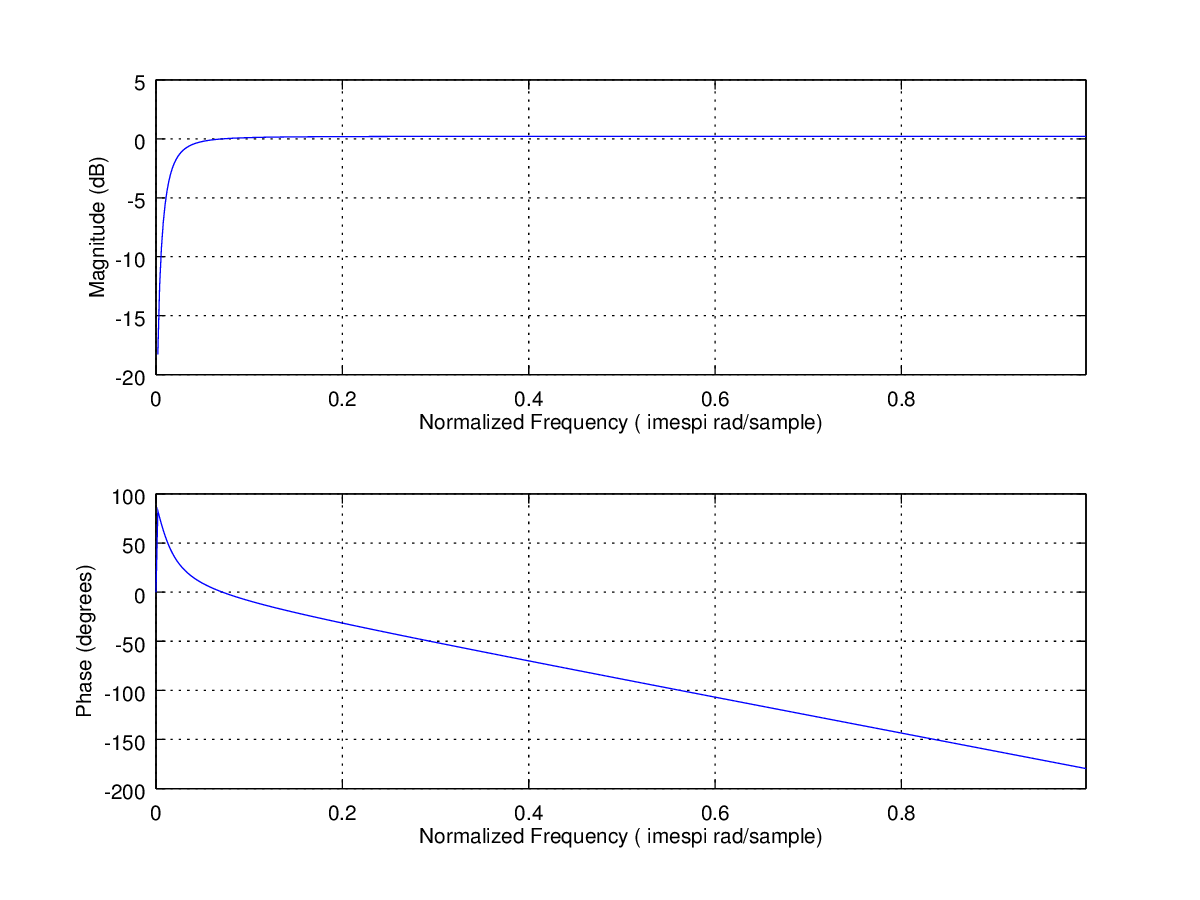
\includegraphics[width=1.0\linewidth]{dc_filter}
			\captionof{figure}{Ideal Filter Magnitude \& Phase Response for $\alpha=.95$}
			\label{fig:ideal}
		\end{minipage}%
		\begin{minipage}{.5\textwidth}
			\centering\captionsetup{type=figure}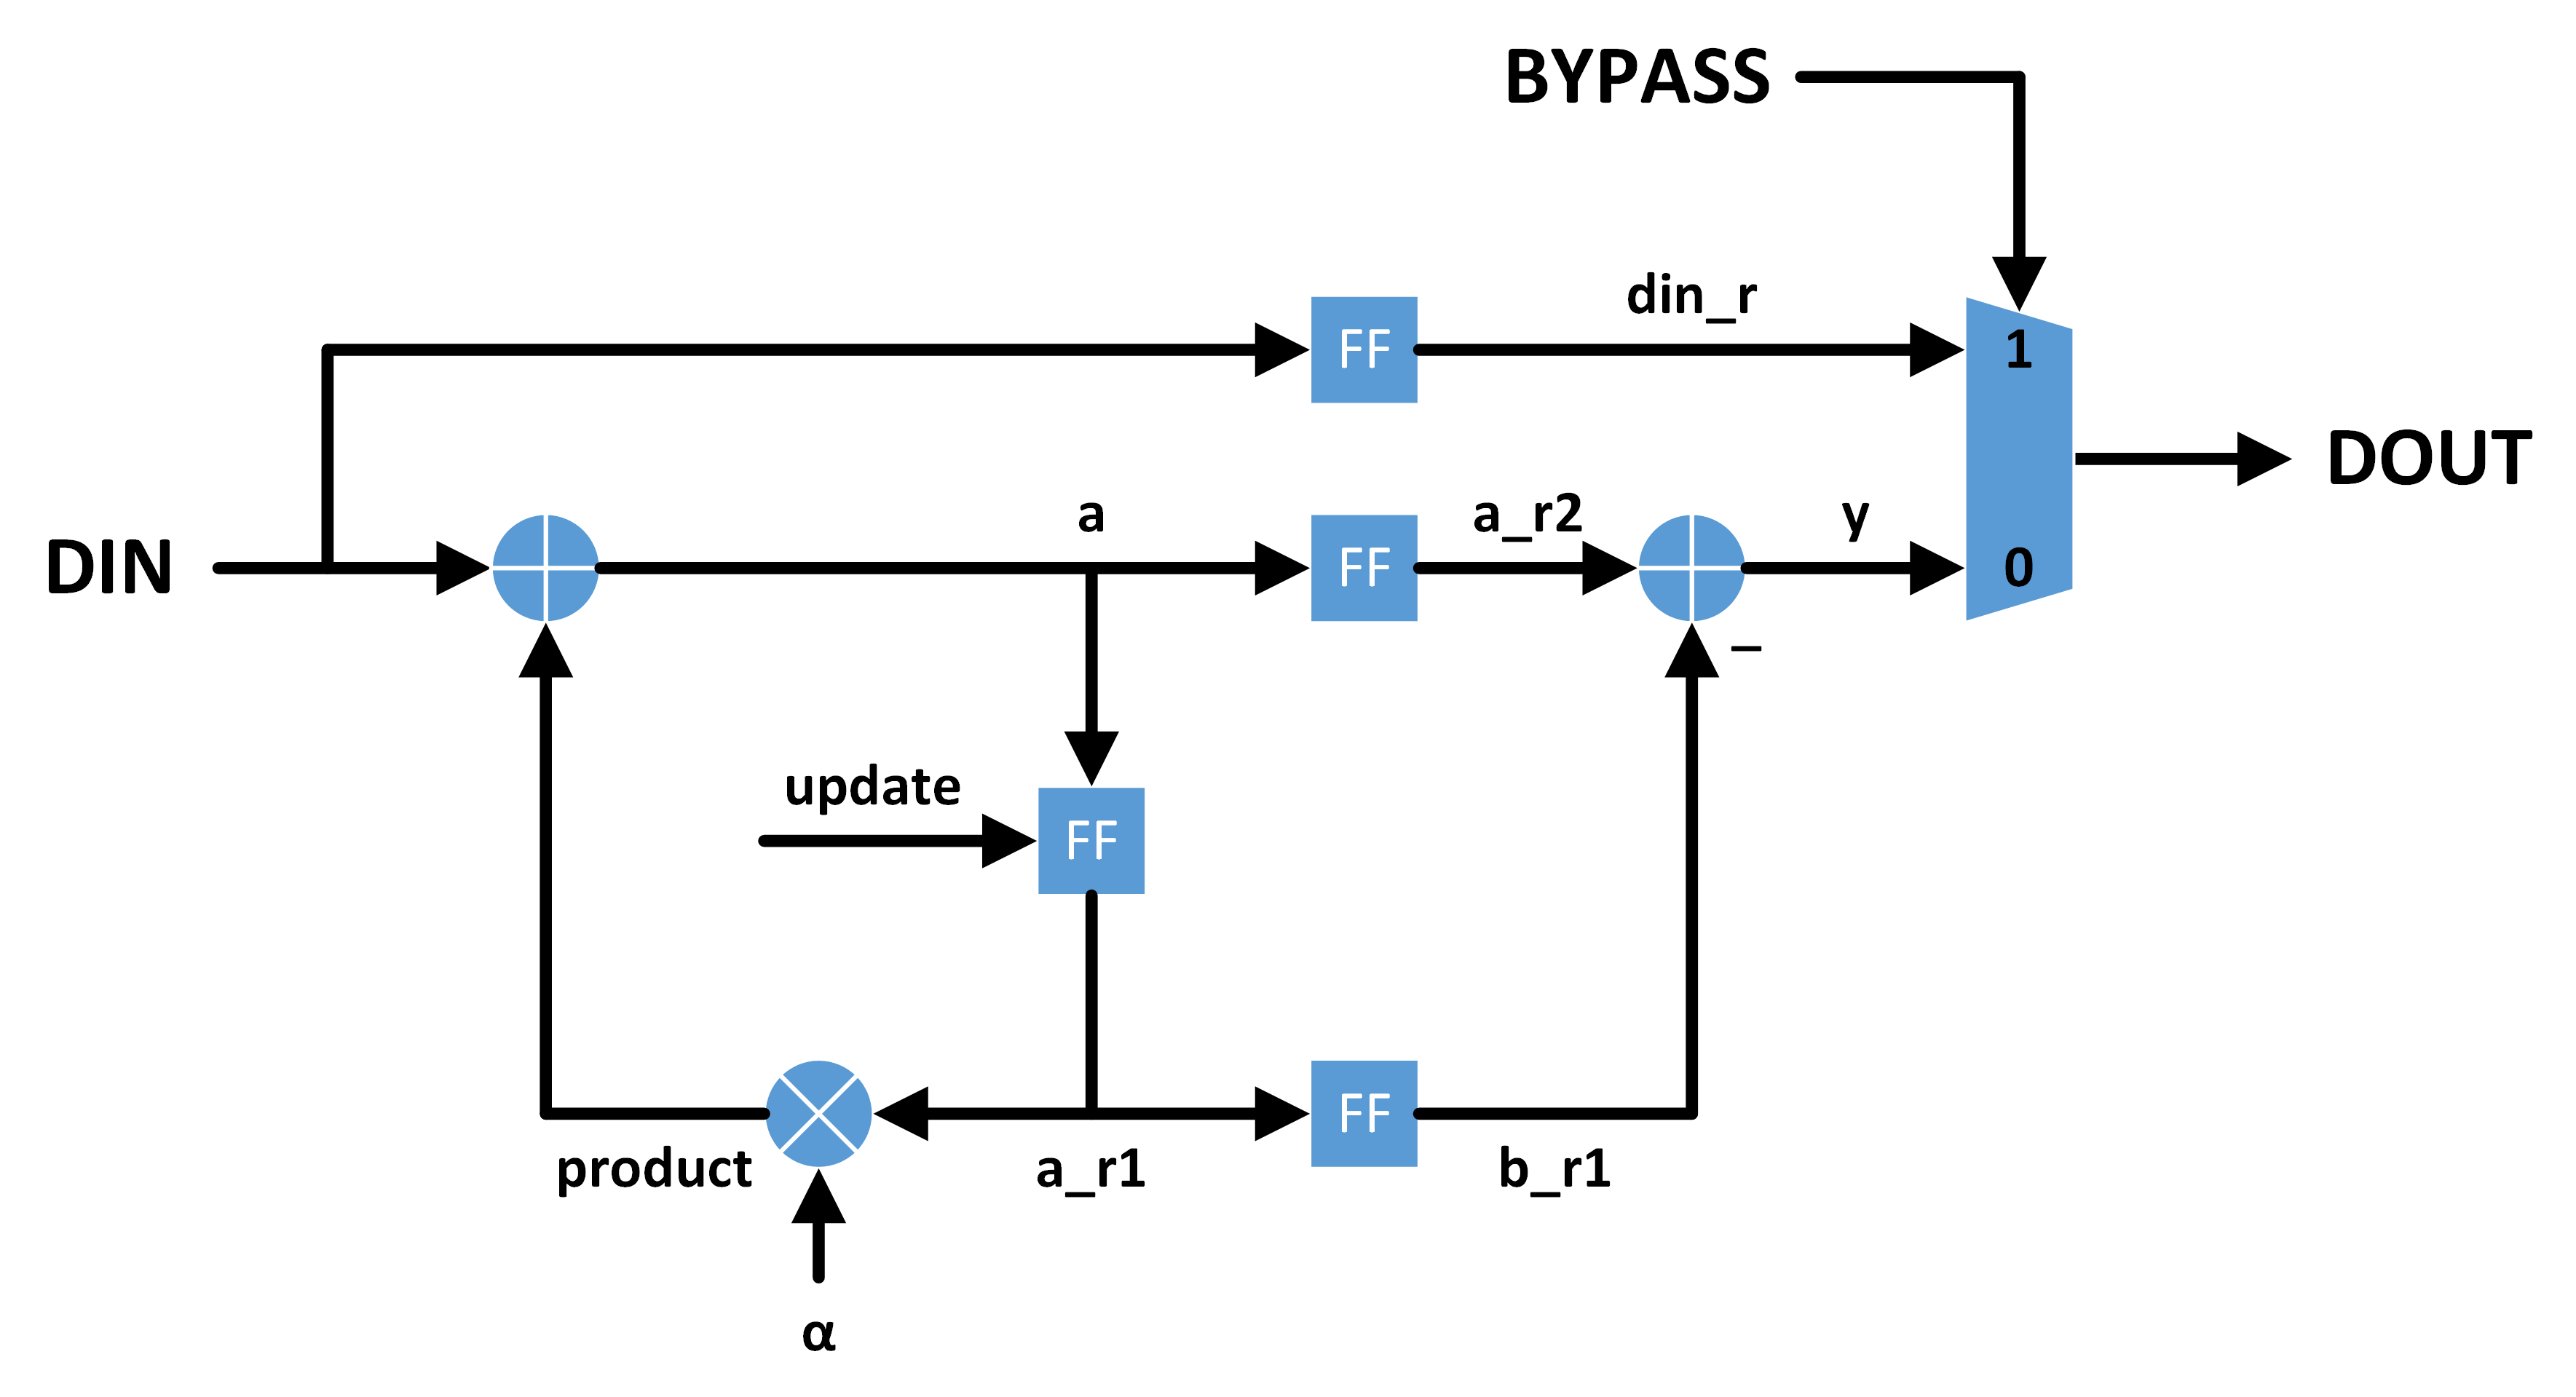
\includegraphics[width=1.0\linewidth]{dc_offset_circuit}
			\captionof{figure}{Circuit Diagram}
			\label{fig:circuit}
		\end{minipage}
	\end{figure}
	The BYPASS input is available to either enable (true) or bypass (false) the circuit. Note that a single bypass register is used, as shown in Figure \ref{fig:circuit} below.\medskip
\end{flushleft}

\section*{Theory}
\begin{flushleft}
	The filter is based upon Richard G. Lyons' ``Understanding Digital Signal Processing, Third Edition'' DC Removal circuit found on Page 761. The text may also be found online here: \href{http://www.embedded.com/design/configurable-systems/4007653/DSP-Tricks-DC-Removal}{DSP-Tricks-DC-Removal}. Lyons' circuit in Figure 13-62d implements the transfer function given in (13-118), which is a 1st-order IIR filter. From Lyons: ``a zero resides at $z=1$ providing infinite attenuation at DC (zero Hz) and a pole at $z=\alpha$ making the magnitude notch at DC very sharp. The closer $\alpha$ is to unity, the narrower the frequency magnitude notch centered at zero Hz.''\medskip

	Adding a delay element to the output, y, does not change the transfer function. Moving the single delay element following the output adder to two delay elements feeding the output adder also does not change the transfer function.\end{flushleft}

	\section*{Block Diagrams}
	\subsection*{Top level}
	\begin{center}
		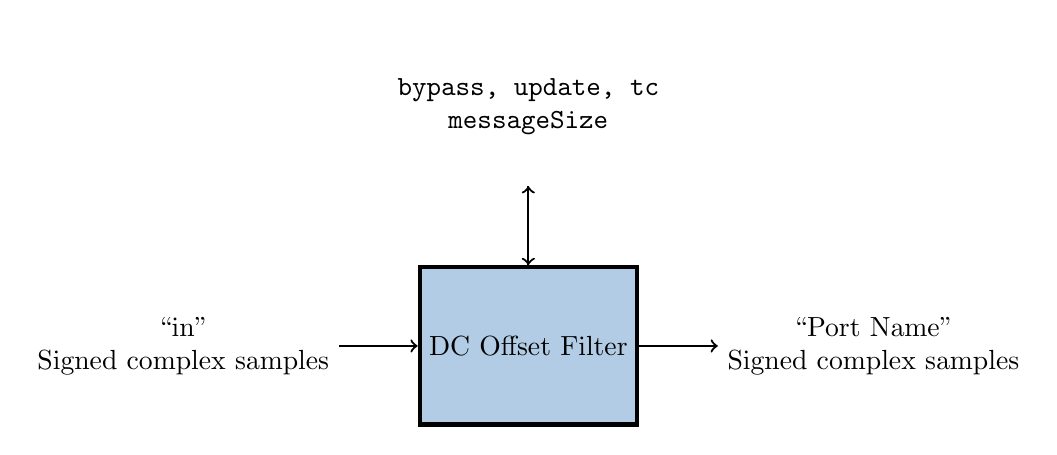
\begin{tikzpicture}[% List of styles applied to all, to override specify on a case-by-case
				every node/.style={
					align=center,  		% use this so that the "\\" for line break works
					minimum size=2cm	% creates space above and below text in rectangle
				},
				every edge/.style={draw,thick}
			]
			\node[rectangle,ultra thick,draw=black,fill=blue](R2){\Comp};
			\node[rectangle,draw=white,fill=white](R3)[left= of R2]{``in'' \\ Signed complex samples};
			\node[rectangle,draw=white,fill=white](R4)[right= of R2]{``Port Name'' \\ Signed complex samples};
			\node[rectangle,draw=white,fill=white](R5)[above= of R2]{\verb+bypass, update, tc+ \\ \verb+messageSize+};
			\path[->]
			(R3)edge []	node [] {} (R2)
			(R2)edge []	node [] {} (R4)
			(R2)edge []	node [] {} (R5)
			(R5)edge []	node [] {} (R2)
			;
		\end{tikzpicture}
	\end{center}
	\newpage

	\subsection*{State Machine}
	\begin{flushleft}
		Only one finite-state machine (FSM) is implemented by this worker. The FSM supports Zero-Length Messages.
	\end{flushleft}
	{\centering\captionsetup{type=figure}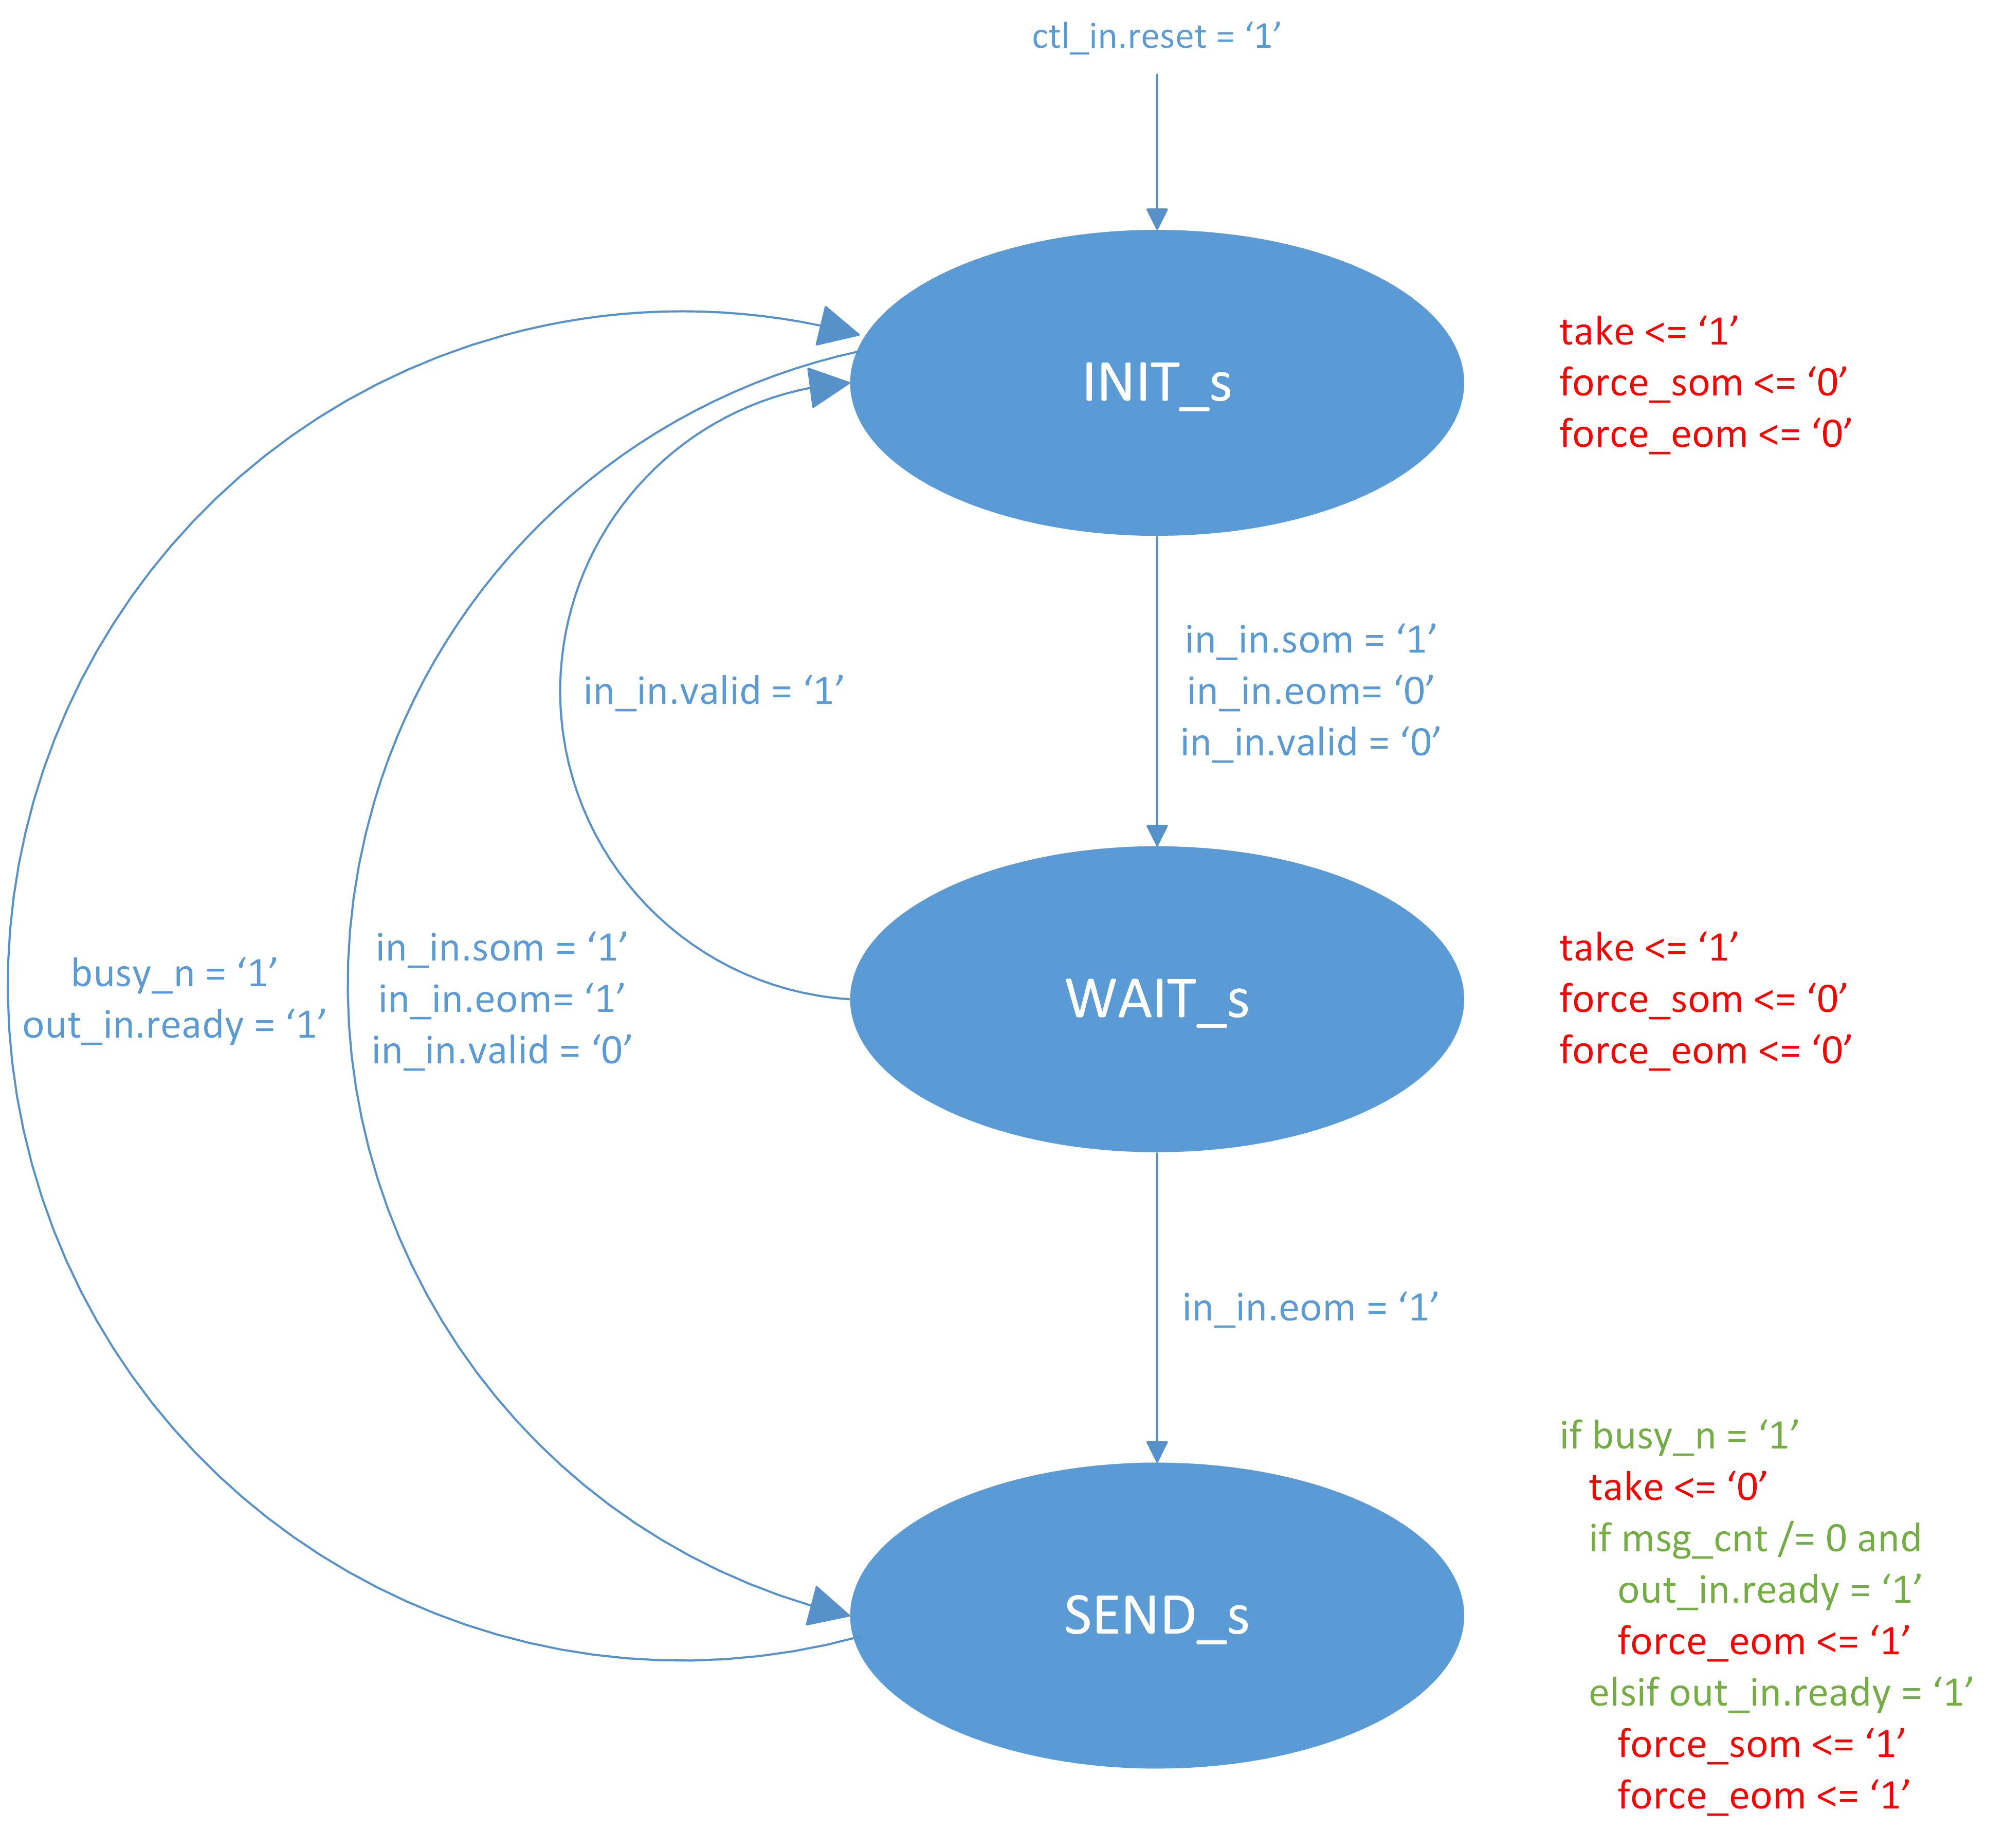
\includegraphics[scale=0.6]{zlm_fsm}\par\captionof{figure}{Zero-Length Message FSM}\label{fig:zlm_fsm}}
	\section*{Source Dependencies}
	\subsection*{\comp.hdl}
	\begin{itemize}
		\item ocpiassets/components/dsp\_comps/dc\_offset\_filter/dc\_offset\_filter.vhd
		\item ocpiassets/hdl/primitives/dsp\_prims/dsp\_prims\_pkg.vhd
		      \subitem ocpiassets/hdl/primitives/dsp\_prims/dc\_offset/src/dc\_offset\_cancellation.vhd
		\item ocpiassets/hdl/primitives/util\_prims/util\_prims\_pkg.vhd
		      \subitem ocpiassets/hdl/primitives/util\_prims/pd/src/peakDetect.vhd
	\end{itemize}

	\begin{landscape}
		\section*{Component Spec Properties}
		\begin{scriptsize}
			\begin{tabular}{|p{3cm}|p{1.5cm}|c|c|c|c|c|p{7cm}|}
				\hline
				\rowcolor{blue}
				Name               & Type   & SequenceLength & ArrayDimensions & Accessibility      & Valid Range & Default & Usage                                                                                                                    \\
				\hline
				\verb+bypass+      & Bool   & -              & -               & Readable, Writable & Standard    & false   & Bypass control                                                                                                           \\					\hline
				\verb+update+      & Bool   & -              & -               & Readable, Writable & Standard    & true    & Update the calculated DC value to be removed, or hold a previously calculated value                                      \\
				\hline
				\verb+tc+          & UChar  & -              & -               & Readable, Writable & 1-127       & 121     & The location of the filter pole along the x-axis between 0 (the origin) and 1 (the unit circle), where $\alpha = tc/128$ \\
				\hline
				\verb+messageSize+ & UShort & -              & -               & Readable, Writable & 8192        & 8192    & Number of bytes in output message                                                                                        \\
				\hline
			\end{tabular}
		\end{scriptsize}

		\section*{Worker Properties}
		\subsection*{\comp.hdl}
		\begin{scriptsize}
			\begin{tabular}{|p{3cm}|p{2cm}|p{1cm}|c|c|c|c|c|p{5cm}|}
				\hline
				\rowcolor{blue}
				Type     & Name                  & Type  & SequenceLength & ArrayDimensions & Accessibility      & Valid Range & Default & Usage                                                    \\
				\hline
				Property & \verb+DATA_WIDTH_p+   & ULong & -              & -               & Readable,Parameter & 1-16        & 16      & Worker internal non-sign-extended data width             \\
				\hline
				Property & \verb+PEAK_MONITOR_p+ & Bool  & -              & -               & Readable,Parameter & Standard    & true    & Include a peak detection circuit                         \\
				\hline
				Property & \verb+peak+           & Short & -              & -               & Volatile           & Standard    & 0       & Read-only amplitude which may be useful for gain control \\
				\hline
			\end{tabular}
		\end{scriptsize}

		\section*{Component Ports}
		\begin{scriptsize}
			\begin{tabular}{|M{2cm}|M{1.5cm}|M{4cm}|c|c|M{9cm}|}
				\hline
				\rowcolor{blue}
				Name & Producer & Protocol           & Optional & Advanced & Usage                  \\
				\hline
				in   & false    & iqstream\_protocol & false    & -        & Signed complex samples \\
				\hline
				out  & true     & iqstream\_protocol & false    & -        & Signed complex samples \\
				\hline
			\end{tabular}
		\end{scriptsize}

		\section*{Worker Interfaces}
		\subsection*{\comp.hdl}
		\begin{scriptsize}
			\begin{tabular}{|M{2cm}|M{1.5cm}|c|c|M{12cm}|}
				\hline
				\rowcolor{blue}
				Type            & Name & DataWidth & Advanced                & Usage                  \\
				\hline
				StreamInterface & in   & 32        & ZeroLengthMessages=true & Signed complex samples \\
				\hline
				StreamInterface & out  & 32        & ZeroLengthMessages=true & Signed complex samples \\
				\hline
			\end{tabular}
		\end{scriptsize}
	\end{landscape}

	\section*{Control Timing and Signals}
	\begin{flushleft}
		The DC Offset Cancellation Filter worker uses the clock from the Control Plane and standard Control Plane signals.
	\end{flushleft}

	\section*{Performance and Resource Utilization}
	\subsubsection*{\comp.hdl}
	\input{../../\ecomp.hdl/utilization.inc}
	\section*{Test and Verification}
	\normalsize
	Two test cases are implemented to validate the \Comp{} component:
	\begin{itemize}
		\item[1)] Normal mode
		\item[2)] Bypass mode
	\end{itemize}
	\noindent For both cases, the input file is a waveform with tones at 5 Hz, 13 Hz, and 27 Hz, and adds a DC bias at 0 Hz. The values are scaled to fixed-point signed 16-bit integers, with a maximum amplitude of 22938 to avoid internal overflow.\par\medskip
	\noindent Time and frequency domain plots may be viewed in Figures \ref{fig:in_time_tone} and \ref{fig:in_freq_tone} below, respectively, where the time domain plot represents the first 128 complex samples in the file.

	\begin{figure}[ht]
		\centering
		\begin{minipage}{.5\textwidth}
			\centering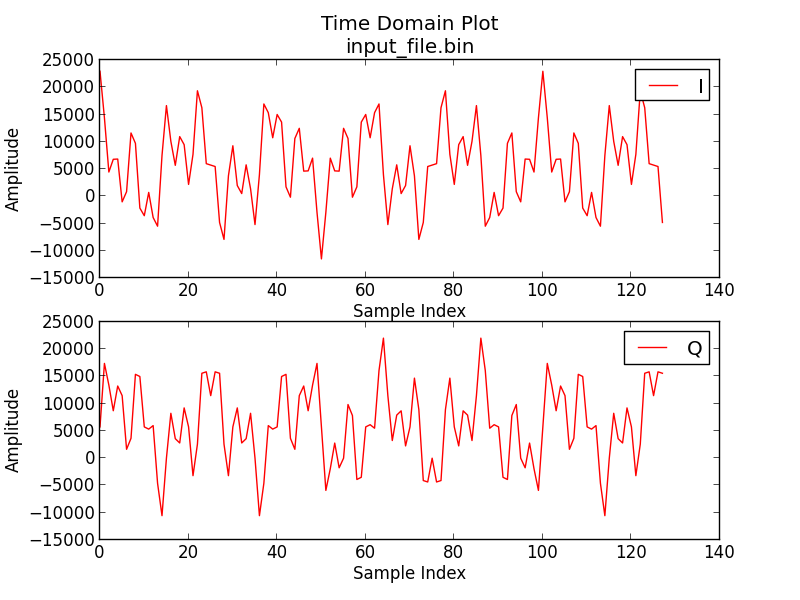
\includegraphics[width=1.0\linewidth]{input_time_tones}
			\captionof{figure}{Time Domain Tones with DC bias}
			\label{fig:in_time_tone}
		\end{minipage}%
		\begin{minipage}{.5\textwidth}
			\centering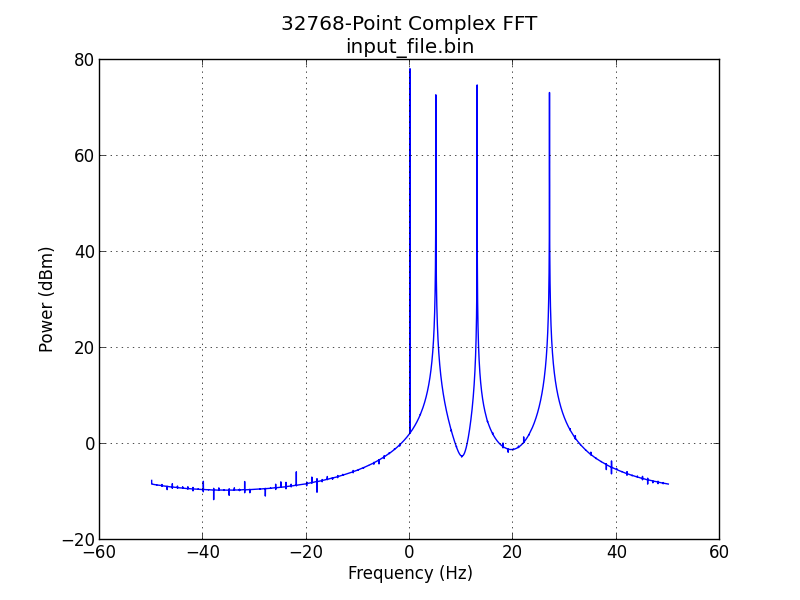
\includegraphics[width=1.0\linewidth]{input_freq_tones}
			\captionof{figure}{Frequency Domain Tones with DC bias}
			\label{fig:in_freq_tone}
		\end{minipage}
	\end{figure}
	\noindent For verification of case 1, the output file is first checked that the data is not all zero, and is then checked for the expected length of 32,768 complex samples. Additionally, both the input and output data are translated to the frequency domain, where a FFT is performed, and then power measurements are taken at DC (zero Hz), 5 Hz, 13 Hz, and 27 Hz. The input and output power measurements are compared to validate that the DC bias has been attenuated and that the other tones have not been attenuated. Figures \ref{fig:out_time_tone} and \ref{fig:out_freq_tone} depict the filtered results of the three tone input. Again, the time domain figure represents the first 128 complex samples in the output time domain file.

	\begin{figure}[ht]
		\centering
		\begin{minipage}{.5\textwidth}
			\centering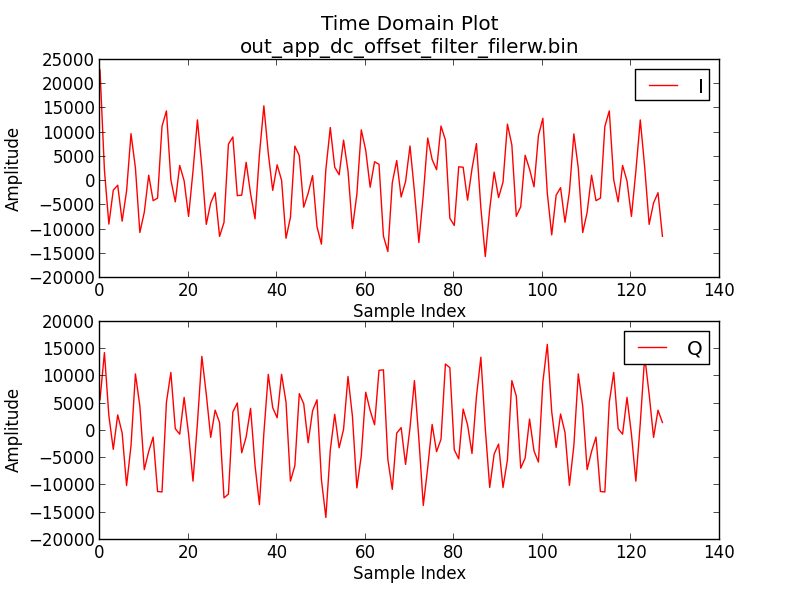
\includegraphics[width=1.0\linewidth]{output_time_tones}
			\captionof{figure}{Time Domain Tones with DC removed}
			\label{fig:out_time_tone}
		\end{minipage}%
		\begin{minipage}{.5\textwidth}
			\centering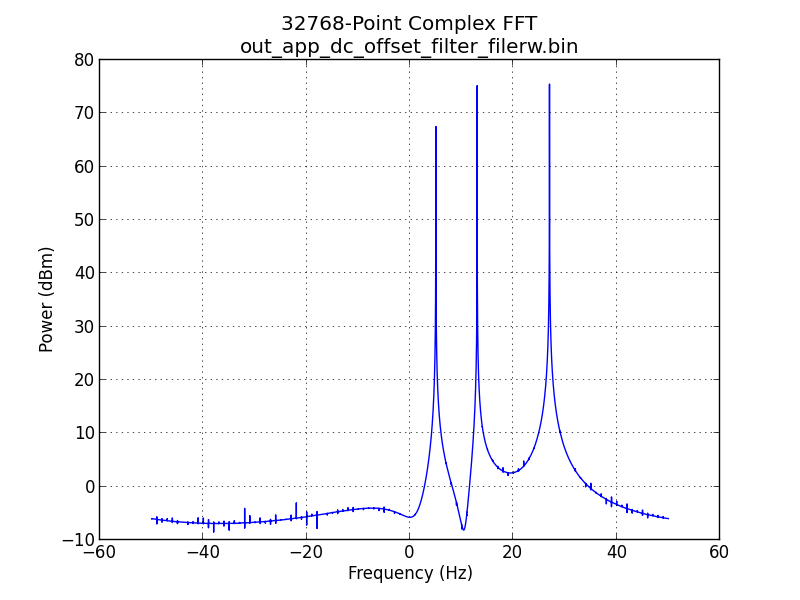
\includegraphics[width=1.0\linewidth]{output_freq_tones}
			\captionof{figure}{Frequency Domain Tones with DC removed}
			\label{fig:out_freq_tone}
		\end{minipage}
	\end{figure}
	\newpage

	\noindent For case 2, the input data is forwarded to the output port. For verification of this case, the output file is byte-wise compared to the input file.
	\section*{References}
	\begin{flushleft}
		\begin{itemize}
			\item[1)] Richard G. Lyons. \textit{Understanding Digital Signal Processing.} Third Edition. Pearson Education, Inc., Boston. 2001.
			\item[2)] Richard G. Lyons. (2008, August 11). \textit{DSP Tricks: DC Removal.} Retrieved from http://www.embedded.com/
			      design/configurable-systems/4007653/DSP-Tricks-DC-Removal.
		\end{itemize}
	\end{flushleft}
\end{document}
